%% name: 日本語論文 (jlreq)
%% desc: jlreq による日本語組版 — 目次・数式・図表・脚注・参照・文献
\documentclass{jlreq}
\usepackage{amsmath}
\usepackage{amssymb}
\usepackage{amsthm}
\usepackage{booktabs}
\usepackage{tikz}
\usepackage[a4paper,margin=25mm]{geometry}

\newtheorem{theorem}{定理}[section]

\begin{document}

\tableofcontents

\section{はじめに}
\label{sec:intro}

ここから書き始めてください。\footnote{脚注もページ下部に罫線つきで
ライブ組版されます。}この文書はLuaTeX-jaによる本物の日本語組版です。
禁則処理と和欧文間スペースが効いた状態で、打鍵に同期してページが
更新されます。図\ref{fig:example}や式\eqref{eq:main}、
文献\cite{knuth84}への参照もすべて編集に追随します。

長い段落でも行分割は本物のアルゴリズムで行われるので、
句読点が行頭に来ることはありませんし、englishとの混植も自然に
処理されます。数式 $e^{i\pi}+1=0$ を文中に置くこともできます。

\section{数式}
\label{sec:math}

\begin{equation}
  \label{eq:main}
  \int_0^\infty e^{-x^2}\,dx = \frac{\sqrt{\pi}}{2}
\end{equation}

\begin{theorem}
  \label{thm:main}
  常駐エンジンにおいて、ページは表示リストのハッシュが変化した
  ときに限りパッチされる。
\end{theorem}

定理\ref{thm:main}の番号は節番号に従属した本物のカウンタです。

\section{図表}
\label{sec:figs}

\begin{figure}[t]
\centering
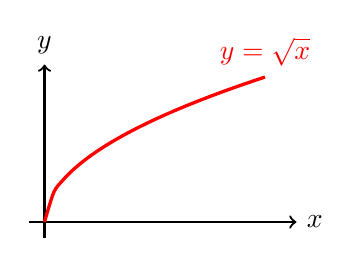
\begin{tikzpicture}[scale=1.0]
  \draw[->, thick] (-0.2,0) -- (3.2,0) node[right] {$x$};
  \draw[->, thick] (0,-0.2) -- (0,2.0) node[above] {$y$};
  \draw[red, very thick, domain=0:2.8, smooth] plot (\x, {sqrt(\x)*1.1})
    node[above] {$y=\sqrt{x}$};
\end{tikzpicture}
\caption{座標を書き換えるとこのブロックだけが再組版されます。}
\label{fig:example}
\end{figure}

\begin{table}[b]
\centering
\begin{tabular}{lrr}
\toprule
項目 & 件数 & 割合 \\
\midrule
甲 & 12 & 40\,\% \\
乙 & 18 & 60\,\% \\
\bottomrule
\end{tabular}
\caption{booktabs罫の表（下部フロート）。}
\label{tab:example}
\end{table}

\section{おわりに}

節\ref{sec:math}で示したとおり、参照・番号はすべてライブです。

\begin{thebibliography}{9}
\bibitem{knuth84} Donald E. Knuth. \emph{The \TeX book}.
Addison--Wesley, 1984.
\bibitem{okumura} 奥村晴彦・黒木裕介『LaTeX2e美文書作成入門』技術評論社.
\end{thebibliography}

\end{document}
